\documentclass[a4paper,11pt]{article}
\usepackage{inputenc}

\usepackage[british]{babel}
\usepackage{amsmath, amssymb, amsfonts}
\usepackage{graphicx, subfig}
\usepackage{natbib}

\usepackage[parfill]{parskip}

\title{A bright future for organic light-emitting transistors}
\author{Cees Draaijer, Armin Palavra \& Ellen Schallig}

\hyphenation{de-ter-mi-ning re-la-tive-ly fab-ri-ca-ting na-no-tubes dom-i-nant tran-sis-tors for-ma-tion ap-pli-ca-tions}

\begin{document}

\maketitle

\section{Kopje koffie}

\textbf{THE introduction!}
Black and Bloom
\section{Relationship to the course (3 to 4 pages)}
Summarize the themes/aspects from the lecture course which are relevant for the paper which you will discuss. 



\subsection{Van Wees}
From the slides, reading material. Van Wees first because he was most fundamental about devices? Building up towards the more advanced organic stuff from Loi (as in the article).



\subsection{Loi}
From the slides, reading material.



\subsection{Tamalika}
Perhaps some historical perspective?


\subsection{LETs based on inorganic semiconductors} %Ellen|Armin

Silicon is the most well known and most successful material in the field of electronics. However, its current use in opto-electronics is limited because of its poor light-emitting properties. This is because silicon is an indirect-bandgap semiconductor, which makes it unfavourable for light emission. For each radiative electron-hole recombination, a phonon is needed to conserve momentum. This causes dominance of non-radiative recombination mainly occurring at lattice defect sites, such as dislocations, impurities, cluster defects and precipitates.

This problem is overcome by using silicon nanocrystals instead of bulk silicon. For nanocrystals hole and electron diffusion is limited by the size of the crystals. This way defect sites become isolated and radiative emission is the dominant recombination pathway. Emission from nanocrystals can therefore be rather high, up to a quantum efficiency of  10\% [ref10]. Additionally, the emitted light can be tuned by the exact size of the nanocrystals, from near-infrared to the visible range. 

To achieve such electrically driven bright emission, an efficient way to inject opposite charges into the nanocrystals is required. The most successful approach has been a FET structure in which nanocrystals are embedded into the gate oxide [ref11]. Electrons and holes are injected by tunnelling through the oxide under application of an alternating electric field. This induces sequential accumulation of electrons and holes in the nanocrystals, and light is generated at each cycle.

In this FET structure the electric field required to generate light is lower than in the LED 'sandwich' structure. This shows why silicon still has great potential to be explored.

However, direct-bandgap inorganic semiconductors are better for applications where opto-electronic performance faces more severe constraints. Materials such as gallium arsenide (GaAs) and indium phosphide (InP) can generate much brighter luminescence and allow higher modulation speeds than silicon. LETs based on an InGaP/GaAs heterojunction have been demonstrated [ref12], showing that LETs based on inorganic semiconductors could be used for display and communication purposes. In a further development the InGaP/GaAs LET was designed as a transistor laser.

Although the performances of inorganic semiconductor LETs and transistor lasers are the best achieved to date, their fabrication process is rather complicated, compatibility with other technology is limited and they are relatively expensive. Hence, it is useful to look at different devices.

\subsection{LETs based on carbon nanotubes} %Armin|Cees

%LET OP: de ~ is voor latex, zo vertellen we dat de punt niet een einde-van-de-zin-punt is maar een afkortingspunt, oftewel niet extra ruimte voor een nieuwe zin invoegen (want erna volgt niet een nieuwe zin).

To prepare nanoscale light sources for use in fully integrated opto-electronic circuits, there are several methods. One of them is the engineering of light-emitting nanowires made of direct-bandgap semiconductors. Duan et al.\ have made advancements in this field by assembling $p$-doped and $n$-doped nanowires to form a $p$--$n$ junction. Gudiksen et al.~achieved this by fabricating nanowire superlattices. Unfortunately for achieving high performance levels, with these methods ease of fabrication is lost as well. %op zich zou dit hele stuk weg kunnen omdat het niet direct over carbon nanotubes gaat, maar over nanowires.

A different approach is to use semiconducting single-walled carbon nanotubes as the active component in a field-effect transistor. Carbon nanotube \textsc{fet}s of $n$-type, $p$-type and ambipolar character have been fabricated. The ambipolar charge transport is achieved by simultaneous injection of holes and electrons via thermally assisted tunnelling through the Schottky barriers formed at the source and drain contacts. Under biasing conditions suitable for ambipolar transport with balanced hole and electron currents, infrared optical emission is generated as the result of electron-hole recombination in the nanotube. This is illustrated in figure~\ref{fig:carbontube}. 

\begin{figure}[!ht]
 \begin{center}
  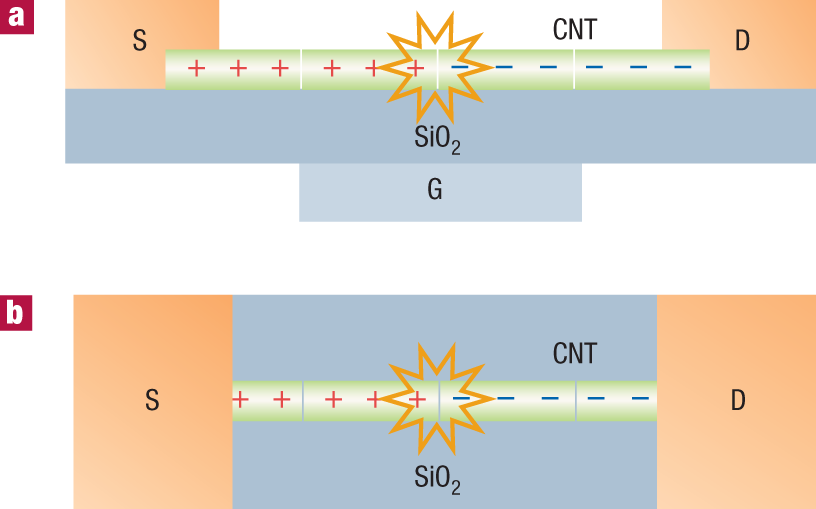
\includegraphics[width=0.6\textwidth]{fig_1}
  \caption{Device structure of a carbon nanotube. (a) Side view. (b) Top view. Infrared emission is generated by the recombination of electrons and holes flowing in the nanotube. From \citet{Muccini}.}
  \label{fig:carbontube}
 \end{center}
\end{figure}

The infrared radiation emitted by the carbon nanotube \textsc{fet} has some special properties. Due to the elongated shape of the tube, the light is polarised parallel to the tube axis. This resembles a linearly polarized dipole radiation source. As the bandgap of the nanotube is inversely proportional to its diameter, it is expected that the wavelength can be tuned by changing diameter sizes. Although this is still to be explored, carbon nanotube \textsc{let}s offer significant potential as nanoscale photon sources that could easily be integrated in opto-electronic devices.


\subsection{LETs based on organic thin films} %Armin|Cees
Some of the most advantageous properties of organic materials used for photoelectronic devices are easy and cheap fabrication. They can for instance be deposited on many different type of surfaces such as a CMOS or cheap materials like plastic and glass. This can result in lower cost devices, especially because organic materials can be produced with low-cost, large scale industrial production processes such as direct printing, ink-jet and other solution based ones. These features make organic thin film devices best suitable for markets were low-cost production is of high importance and the requirements for high performance do not require inorganic devices. (moet/kan nog een stukje tussen over bron 22-25)

OLEDs are very well known and widely used in low-voltage-driven light-emitting devices, possibly produced on flexible substrates. Where OLETs could produce electroluminescence with the same materials al OLEDs the driving scheme behind it is very different. The main difference is that charge transport in OLEDs occurs perpendicular and through the plane of different layers. Whereas in OLETs charge transport occurs parallel and through the plane. An schematic representation is shown in figure xx. For the OLEDs the charge transport is bulk charge transport, for the OLETs it is field-effect charge transport [26]. An other large difference is the distance the minority carriers are required to travel before encountering a charge of the opposite sign and recombine radiatively. In OLEDs the distance the charges have to travel are in the order of few tens of nanometers where for a typical ambipolar OLET the distance is in the order of hundreds nanometers or a few micrometers. This larger distance requires stricter charge transport properties of materials. (iets met electroluminces quantum efficiency). Due to the device structure (the spacial distance between the exciton formation region and the metal electrodes is much larger in OLETs), OLETs are less affected by electron-metal quenching by interaction with charge carriers. This effect is further reduced by the availability of a third electrode that balances electron and hole currents. These structural advantages make OLETs more favourable for high-brightness electroluminescence and highly integrated devices. These advantages however do rely on development of organic materials.

\subsection{Unipolar OLETs} %Cees|Ellen

OLETs were first demonstrated by Hepp et al. using a tetracene thin film. Tetracene is the four-ringed member of the series of acenes, a class of organic compounds and polycyclic aromatic hydrocarbons made up of linearly fused benzene rings. Moreover, it is a molecular organic semiconductor. Typical current carriers in organic semiconductors are holes and electrons in π-bonds. Almost all organic solids are insulators. But when their constituent molecules have π-conjugate systems, electrons can move via π-electron cloud overlaps, especially by hopping, tunnelling and related mechanisms. Also polycyclic aromatic hydrocarbons work with this mechanism.

To make the first OLET, Hepp used interdigitated gold source and drain electrodes, fabricated on a Si/SiO2 substrate before deposition on the organic active layer. The charge transport and light emitting layer is the tetracene, configured as a polycrystalline film. The resulting electrical characteristics are typical for a p-type FET. Light emission from the tetracene indicates that electrons and holes are simultaneously injected into the active layer. The electrons can not move through the tetracene, so that they are trapped at the gold/tetracene interface. At this interface they then recombine with the holes, emitting light.

One important issue that can be relevant for other materials under the same driving scheme is that electrons are injected from gold into tetracene over a (from basic principles unexpected?) nominal barrier of 2.7 eV. This points to the actual structure of the gold/tetracene interface, where a composite layer could be formed. Thus it is no simple matter of considering the different materials' energy levels separately. 

A number of investigations were done to optimize this first device and to make it ambipolar. Yet never electron transport was observed in the tetracene thin films. The primary limiting process for achieving (the then resulting?) high-brightness emission is singlet-triplet quenching. This was concluded after numerical simulations looking at exciton processes. Triplets appear to be most dominant in quenching singlets. This prevents pure tetracene films, when provided with a realistic optical feedback structure, to reach the threshold for (the desired?) stimulated emission.

OLETs electroluminescent and electrical properties are, among other things, dependent on the transistor channel length. On decreasing the channel length, both electron injection and electro-luminescence efficiency are improved. This unfortunately holds up to a certain point. Scaling down the channel further the contact resistance from a typical metal/organic interface tends to dominate the electrical characteristics of the transistor, hindering further improvement. Unfortunately the external quantum efficiency is still very low, so that there are no practical applications. 

Organic materials with both efficient electroluminescense and transistor characteristics are needed. The application of well-established OLED materials is not straightforward, as most of them have low FET-performance. Their strong molecular packing that allows high-mobility, increases non-radiative decay.

As an alternative spin-coated polymers have been used as active layers in LETs with bottom-contact device structures as in Figure B1 in the case study article. The polymers used are among the most commonly used LED polymers. In addition to extending OLET concepts to polymers, experiments show a clear increase in light-emission efficiency on using metals for source and drain electrodes that have a workfunction more suitable for holes and electrons injections respectively (that's like totally you opinion dude, even uitleggen!).

As mentioned before, to fabricate large-area and low-cost devices, the good solubility of the organic semiconductor, which would allow printing and casting processes, is important. A new molecular system was devised which is suitable for drop-casting onto a pre-patterned FET structure to produce OLET devices. Although the transistor characteristics are less than if produced by vacuum sublimation, most likely due to morphological characteristics of the solution-processed films and to the lower degree of molecular ordering, it widens the range of processing techniques and again points to the crucial role played by synthetic chemistry in tailoring the processing conditions and functional properties of materials.
\subsection{Ambipolar OLETs} %Cees|Ellen
In unipolar devices only one type of charge carrier is transported efficiently across the transistor channel and light generation is restricted to an area close to the minority carrier injection electrode. Ambipolar organic semiconductor devices don not have this limitation. This means that they can be fabricated of complementary logic circuits with a single active layer. Ambipolar charge transport is crucial in LETs for maximizing exciton recombination through electron-hole balance as well as for adjusting the position of the recombination region in the channel by tuning the gate voltage. The consequent decrease of exciton quenching leads to improved quantum efficiency of the emission from the device.

In principle, pure organic semiconductors should support both electron and hole conduction equally. However in practice most of the organic semiconductor films only display unipolar charge transport. Of these the majority is p-type, so holes are more mobile than electrons). Ambipolar field-effect charge mobility of electroluminescent organic thin films seems to be limited and their optoelectronic response in a device structure remains to be explored.

For instance, as the field-effect mobility determines the switching time of the OLET device and is a critical parameter for all those applications where light emission is to be modulated by the applied voltage, e.g. for active matrix displays and frequency-modulated nano-scale light sources.

In view of the limited number of electroluminescent materials with good ambipolar mobility values, alternative approaches to achieve high ambipolar transport in OLETs have been explored. The first ambipolar OLETs were demonstrated using a bulk heterojunction as the active component of the device. Like previously applied in LEDs, solar cells and FETs, this uses the mixing of two materials with complementary properties.

The most important requirement that the two materials must comply with, is that the relative positions of the HOMO and LUMO must allow exciton formation and recombination in the material with the smaller energy gap. Given this restriction, the approach of the bulk heterojunction can be extended to other materials in the search for higher-brightness OLET devices). The electroluminescense intensity is also determined by the relative concentration of materials and by the structural features of the bulk heterojunction. However, the absolute mobility values are low.

OLETs based on two component layered structures have been realized. Here growth compatibility between the n-type and p-type materials is essential in forming a continuous interface and in controlling the resulting optoelectronic response of the OLET. Therefore the sequence of the deposition of the layers is important for determining the device characteristics. The optimum performance is not necessarily achieved by using materials with the highest mobility values in single-layer devices. 

To date, the bilayer approach provides the highest balanced mobility values in ambipolar OLET devices. However the separation between the electron transport layer and the hole transport layer, in spite of the electron-hole attraction, drastically reduces the probability of electrons and holes meeting to form excitons inside the device channel. When charges are accumulated at the interface between the dielectric substrate and the organic material, near the drain top electrode, the superposition of gate contact/bilayer/drain contact is likely to form an LED structure at the origin of the light emission, which is therefore confined next to the drain metal electrode as in the case of unipolar OLETs.

Recently it was shown that in the polymer-based ambipolar LETs the emission zone can be scanned across the transistor channel on changing the gate bias. This was done with low-workfunction metals for the electron-injection electrode and of a high-workfunction metal for the hole-injection electrode. In addition, trap-free dielectrics were used to avoid electron trapping and enable ambipolar transport. 

The observation of a spatially resolved recombination zone whose location in the transistor channel is controlled by the applied bias, demonstrates the coexistence of electron and hole channels, and therefore the ambipolar nature of charge transport. The recombination zone is located at the centre of the channel when electron and hole currents are balanced. The electroluminescense quantum efficiency can be as high as that of LEDs based on the same material. 

At present, the drawback of the ambipolar polymer-based LETs remains the mobility values. However, the latest results, together with the continuous development of the knowledge of the chemical/physical properties of the relevant interfaces in the device, and the possibility of chemically tailoring the active materials, open exciting perspectives for the full realization of the scientific and technological potential of OLETS.





\subsection{Directions and opportunities} %Ellen|Armin

\textsc{olet}s are of high interest as they can be used in many different applications, from communication systems to solid-state lighting, and provide a novel device architecture to investigate fundamental optoelectronic properties in organic materials. The in-plane architecture of \textsc{olet}s allows for direct probing and observation of various fundamental aspects of organic material science, as opposed to the \textsc{oled} technology.

\textsc{olet}s may be the key element for the next-generation organic active matrix display technology. They can provide effective solutions for the brightness and lifetime of the electroluminescent pixels, through the high degree of control of charge injection and accumulation in the organic layer. The integration of light-emitting and electrical switching in one element reduces the amount of other elements to be produced, which results in a cheaper fabrication of the active matrix display.

The in-plane \textsc{olet} structure can be a valid alternative for the vertical \textsc{oled} structure for an electrically pumped organic laser. These lasers have many advantages over the III-V semiconductor lasers, such as lower cost and wider range of possible lasing emission. However exciton quenching and photon losses are still major problems, which have prevented the realization of the electrically pumped organic laser to date.

The \textsc{let} configuration can prevent exciton quenching and photon losses by moving the metal electrodes away from the region of exciton formation and light emission. The high mobility of carriers in a \textsc{fet} configuration minimizes the required charge-carrier densities, which also reduces exciton quenching and photon absorption. These key advantages make the field-effect transistor approach the most favourable for achieving the organic laser.

\textsc{olet}s have potentially higher light-emission efficiency and brightness than \textsc{oled}s, which opens the market of low power consumption solid state lighting. \textsc{olet}s also can be fully compatible with well-established other technologies which may allow for the development of optical communication with \textsc{olet}s as a key active element. Finally, \textsc{olet}s can be solution processed and fabricated on plastic surfaces. This is a gateway for the printing on large-area and flexible substrates.
	

\section{Summary: importance/relevance of the devices}

Given the title of the article, ``A bright future for organic field-effect transistors", it is clear that the devices in general sense are deemed very important. Yet there is still a lot of work to be done, so that the article has to differentiate in different device generations and design concepts. There is an important role for synthetic chemistry in tailoring the processing conditions and functional properties of materials. In many cases there is a trade-off between high-performance and ease of fabrication.

The general objective is to allow the fabrication of multifunctional organic devices using extremely simple device structures. This has strong economical relevance. OLETs represent a step forwards. As compared to OLEDs, a clear advantage is their potentially higher electroluminescence quantum efficiency. Moreover they can be used to investigate fundamental optoelectronic properties in organic materials, and can be used in all kinds of applications, ranging from display technology to electrically driven organic lasers. In these applications they may enable the development of next-generation technologies, such as organic active matrix display technology.

The full-compatibility of OLETs with many well-established electronic and photonic technologies, makes that they can have a huge impact. Especially because they can be fabricated on plastic substrates in combination solution processing. This enables relatively low-cost production, so that also the economic drivers are huge.
\section{Future applications (1/2 page)}
4) Give suggestions for future applications/improvement and/or further research of the devices . Other comments are also possible (for example if you think that the devices are not useful)   (about � page). Nature even scannen ofzo


\bibliographystyle{plainnat}
\bibliography{bibliography}
\end{document}
